\section{handrobotic}
perintah navigasi directori

\section{membuat tangan pemindah barang berdasarkan warna}
Dibuat berdasarkan penelitian intership1 sampai dengan TA.

\section {ARM robot/hand robotic}
Teknologi robotika berkembang pesat sering meningkatnya kebutuhan robot cerdas. Kata robot sudah tidak asing lagi di telinga kita. Kata robot berasal dari bahasa Czezh, robota yang berarti ‘bekerja’. Kata robot diperkenalkan oleh karel Capek saat mementaskan RUR (Rossum’s Universal Robots) pada tahun 1921.Awal kemunculan robot dapat ditesuri dari bangsa yunani kuno yang membuat patung dapat di pindah-pindahkan. Sekitar 270 BC, Ctesibus, seorang insinyur Yunani, membuat organ dan jam air dengan komponen yang dapat dipindahkan. Pada zaman Nabi Muhammad SAW, telah dibuat mesin perang yang menggunakan roda dan dapat melontarkan bom. Bahkan, Al-Jajari (1136-1206) seorang ilmuwan Islam dinasti Artuqid yang dianggap pertama kali menciptakan robot humanoid yang berfungsi sebagai 4 musisi.

Pada tahun 1770, Pierre Jacquet Droz, Seorang pembuat jam berkebangsaan Swiss membuat 3 boneka mekanis. Uniknya, boneka tersebut dapat melakukan fungsi spesifik, yaitu mnulis. Boneka yang lain dapat memainkan musik dan menggambar. Pada tahun 1898, Nikola Tesla membuat sebuat boat yang dikontrol melalui radio remote control. Boat ini didemokan di Madison Square Garden, Nmaun, usaha untuk membuat autonomus boat tersebut gagal karena masalah dana.

	Pada tahun 1967, Jepang mengimpor robot Versatran dari AMF. Awal kejayaan robot berawal pada tahun 1970, ketika profesor Victor Scheinman dari Universitas Standford mendesain lengan standart. Saat ini, konfigurasi kenematiknya dikenal sebagai standart lengan robot. Terakhir, pada tahun 2000, Honda memamerkan robot yang dibangun bertahun-tahun lamanya bernama ASIMO, serta diusul oleh sony dengan robot AIBO. 

\section{Teori mengenai warna}
Warna Adalah Sebuah sensasi yang dihasilkan ketika suatu energi cahayamengenai suatu benda, dimana cahaya tersebut akan di refleksikan atau ditransmisikan secara langsung oleh benda yang terkena cahaya tadi dan cahayayang di refleksikan atau di transmisikan tersebut yang akan dilihat oleh mata pengamat. Ada dari istilah warna Istilah lain yang dikenal dalam warna adalah nilai warna. Nilai warna dapat ditentukan dari tingkat kecerahan ataupun tingkat kesuraman sebuah warna. Nilai ini dipengaruhi oleh penambahan putih maupun hitam. Dalam suatu sistem RGB, nilai ditentukan dari penambahan komponen merah, biru, dan juga hijau dalam sebuah komposisi yang tepat dan sama meskipun tidak harus berjumlah 100 persen.

\section{Warna RGB}
Warna RGB merupakan  model warna yang bersifat additive. Di mana RGB berguna sebagai  alat penginderaan dan presentasi gambar pada tampilan visual peralatan elektronik seperti komputer dan televisi. RGB sendiri merupakan singkatan dari : R = Red (Merah), G = Green (Hijau), dan B = Blue (Biru). Ketiga warna dasar ini berfungsi untuk berbagi intensitas cahaya untuk mencerahkan warna latar yang gelap (hitam).  Warna RGB difungsikan untuk tampilan monitor peralatan elektronik seperti komputer karena latar belakang warna monitor komputer adalah hitam.

\section{Motor servo}
Motor Servo adalah sebuah motor DC kecil yang diberi system gear dan potensiometer sehingga dapat menempatkan “hom’ servo pada posisi yang di kehendaki. Motor servo ini jelas menggunakan system loop sehingga posisi “hom” yang dikehendaki bisa dipertahankan. Motor servo biasa digunakan untuk robot berkaki, lengan robot atau sebagai actuator pada mobil robot. Motor servo terdiri dari sebuah motor DC, beberapa gear, sebuah potensiometer, sebuah output shaft dan sebuah rangkaian control elektronik. seperti pada gambar\ref{fig_handrobotic}
\begin{figure}[!htbp]
  \centering
  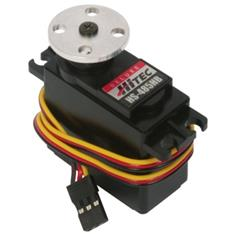
\includegraphics[width=0.45\textwidth]{figures/handrobotic/motorservo.jpg}
  \caption{berikut ini adalah salah satu contoh motor servo}\label{fig_handrobotic}
\end{figure}

\section{Fuzzy logic control}
Fuzzy logic control adalah suatu sistem pengendalian yang memanfaatkan logika fuzzy. Logika fuzzy sendiri dipahami sebagai suatu proses pengambilan keputusan berbasis aturan yang bertujuan untuk memecahka nmasalah, dimana system tersebut sulit untuk dimodelkan atau terdapat ambiguitas dan ketidakjelasan. Itu sebabnya Logika Fuzzy juga disebut sebagai logika kabur atau samar karena logika fuzzy menangkap informasi-informasi yang tidak pasti menjadi nilai-nilai logika yang harus diperhitungkan.
